\documentclass[border=4pt]{standalone}
\usepackage{amsmath,amssymb,amsfonts}
\usepackage{xcolor,colortbl,array,booktabs,multirow}
\usepackage{tikz}
\usepackage{pgfplots}
\pgfplotsset{compat=1.16}
\usetikzlibrary{arrows, automata, backgrounds, calendar, chains, decorations,
    matrix, mindmap, patterns, petri, positioning, shadows, shapes.geometric,
    trees, shapes, decorations.pathreplacing, calc, tikzmark, arrows.meta,
    intersections, fit, graphs, quotes, angles, decorations.markings}
\newcommand{\st}{\text{ s.t. }}
\newcommand{\x}{\mathbf{x}}
\renewcommand{\b}{\mathbf{b}}
\renewcommand{\c}{\mathbf{c}}
\newcommand{\A}{\mathbf{A}}
\newcommand{\y}{\mathbf{y}}
\newcommand{\z}{\mathbf{z}}
\newcommand{\R}{\mathbb{R}}
\newcommand{\RR}{\mathbb{R}}
\newcommand{\Z}{\mathbb{Z}}
\newcommand{\ZZ}{\mathbb{Z}}
\newcommand{\npcomplete}{NP-complete}
\providecommand{\true}{\text{TRUE}}
\providecommand{\false}{\text{FALSE}}
\tikzset{vertex/.style={circle,fill=black!25,minimum size=20pt,inner sep=0pt},
    edge/.style={draw,thick,-},weight/.style={font=\small},
    selected vertex/.style={vertex, fill=red!24},
    selected edge/.style={draw,line width=2pt,-,red!50},
    ignored edge/.style={draw,line width=2pt,-,black!20}}
\newcommand{\vect}{\vec}
\providecommand{\ds}{\displaystyle}
\providecommand{\longvect}{\overrightarrow}
\usepackage[normalem]{ulem}
\definecolor{ocre}{RGB}{243,102,25}
\providecommand{\leftB}{\left[}
\providecommand{\rightB}{\right]}
\tikzset{directed/.style={postaction={decorate,decoration={markings,mark=at position .65 with {\arrow{>}}}}},
    directed1/.style={postaction={decorate,decoration={markings,mark=at position .65 with {\arrow{>}}}}}}
\begin{document}
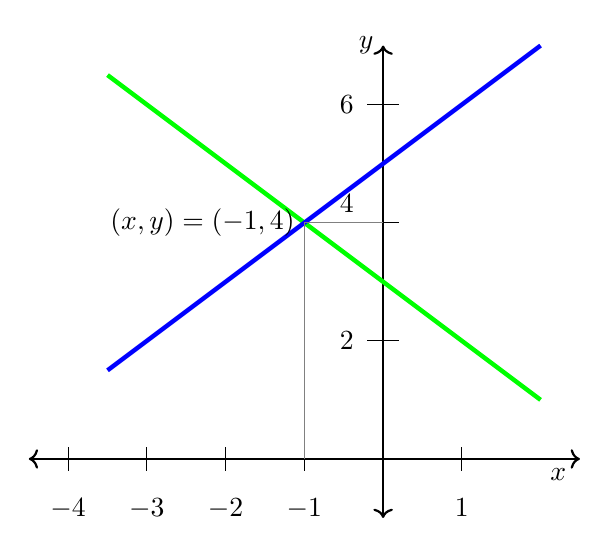
\begin{tikzpicture}[yscale=0.75]
\draw[thick, <->](-4.5,0) -- (2.5,0);
\draw[thick, <->](0,-1) -- (0,7);
\draw(-4,-0.2) -- (-4,0.2);
\draw(-3,-0.2) -- (-3,0.2);
\draw(-2,-0.2) -- (-2,0.2);
\draw(-1,-0.2) -- (-1,0.2);
\draw(1,-0.2) -- (1,0.2);
\draw(-0.2,2) -- (0.2,2);
\draw(-0.2,4) -- (0.2,4);
\draw(-0.2,6) -- (0.2,6);
\draw[green, ultra thick, domain=-3.5:2] plot (\x, {3-\x});
\draw[blue, ultra thick, domain=-3.5:2] plot (\x, {\x+5});
\draw[help lines](-1,0)--(-1,4)--(0,4);
\node[below] at (-4,-0.5){$-4$};
\node[below] at (-3,-0.5){$-3$};
\node[below] at (-2,-0.5){$-2$};
\node[below] at (-1,-0.5){$-1$};
\node[below] at (1,-0.5){$1$};
\node[left] at (-0.25,2){$2$};
\node[above left] at (-0.25,4){$4$};
\node[left] at (-0.25,6){$6$};
\node[below right] at (2,0){$x$};
\node[left] at (0,7){$y$};
\node[left] at (-1,4){$(x,y) = (-1,4)$};
\end{tikzpicture}
\end{document}
